\documentclass[10pt]{article}

\usepackage{html}
\usepackage{graphicx}

\newcommand{\mysection}[1]{\section{#1}\label{#1}}
\newcommand{\mysubsection}[1]{\subsection{#1}\label{#1}}
\newcommand{\mysubsubsection}[1]{\subsubsection{#1}\label{#1}}
\newcommand{\remark}[1]{[\emph{#1}]}

\begin{document}

\title{
{\html {\htmladdnormallink{Ibis} {http://www.cs.vu.nl/ibis/}}}
{\latex {Ibis}}
Programmer's Manual}

\author{The Ibis Group}

\maketitle

\section{Introduction}

Ibis is an efficient and flexible Java-based programming environment for Grid
computing, in particular for distributed supercomputing applications.
This manual describes how to write and run Ibis applications.
\html{
It is also available in
\htmladdnormallink{postscript}{http://www.cs.vu.nl/ibis/progman.ps.gz}.}
\latex{It is available on-line at http://www.cs.vu.nl/ibis/progman.}
Ibis is described in several publications (see Section \ref{Further Reading}).
Rather than giving a detailed overview of what each class and method does,
the aim of this document is to describe how to actually use these classes
and methods.
The \emph{docs/api} subdirectory of the Ibis installation provides
documentation for each class and method (point your favorite browser
to docs/api/index.html file of the Ibis installation).
The Ibis API is also available
\html{\htmladdnormallink{on-line}{http://www.cs.vu.nl/ibis/api}.}
\latex{on-line at http://www.cs.vu.nl/ibis/api}.
In this manual, fragments of an actual Ibis application will be used for illustration purposes.
Section \ref{An Ibis Application} will discuss a typical Ibis application,
with subsections on each phase of the program.
Section \ref{Compiling and Running an Ibis Application} will discuss how to
actually compile and run this program.

We also built several systems on top of Ibis.
Section \ref{The Satin Divide-and-Conquer System}
gives an overview of the Satin divide-and-conquer
system, and Section~\ref{gmi-sec} discusses GMI
(Group Method Invocation),
a flexible group communication system.
We also built a RMI (Remote Method Invocation)
implementation on top of Ibis. RMI documentation can be found at
{\html {\htmladdnormallink{http://java.sun.com/j2se/1.4.2/docs/guide/rmi}{http://java.sun.com/j2se/1.4.2/docs/guide/rmi}}}
{\latex {http://java.sun.com/j2se/1.4.2/docs/guide/rmi}}.
Section \ref{Ibis RMI} briefly discusses the Ibis RMI implementation.

\mysection{Some Ibis concepts}

\mysubsection{The Ibis Portability Layer}

An important part of the Ibis system consists of the Ibis Portability Layer (IPL).
The IPL consists of a set of Java interfaces and classes that define how an Ibis application
can make use of the Ibis components.
The Ibis application does not need to know which specific Ibis implementations are
available.
It just specifies some properties that it requires, and the Ibis system
selects the best available Ibis implementation that meets these requirements.
 
\mysubsection{An Ibis Instance}

A loaded Ibis implementation is called an \emph{Ibis instantiation}, or 
\emph{Ibis instance}.
An Ibis instance is identified by a so-called
\emph{Ibis identifier}.
An application can find out which Ibis instances are present in the run
by supplying a so-called \emph{ResizeHandler}.
This ResizeHandler is an object with, among others, a \texttt{joined()}
method which gets called by the Ibis system when a new Ibis instance
joins the run.  The Ibis identifier of this new Ibis is a parameter
to the \texttt{joined()} method.

\mysubsection{Send Ports and Receive Ports}

The IPL provides primitives to communicate between send and receive ports.
In general a connection can be between multiple send ports and multiple
receive ports, but the user may specify that a connection will have only
a single send or receive port, allowing Ibis to choose a more efficient
implementation.  A connection is always \emph{unidirectional}; reverse
connections are conceptually totally independent.

All send and receive ports have a \emph{type} which is represented by an
instance of \texttt{ibis.ipl.PortType}.
To create a connection, an Ibis application requests new send and receive
ports from such a port type, and requests that a connection is set up 
between these ports.

To send a message, the Ibis application requests a new write message from
a send port, puts data in this write message using the provided methods,
and invokes the \texttt{finish()} method to send the message.

To receive a message, the IPL provides two mechanisms:
\begin{description}
\item[explicit receipt]
when a receive port is configured for explicit receipt, a message can be
received with the receive port's blocking \emph{receive} method,
or with its non-blocking \emph{poll} method.
These methods return a \emph{read message} object, from which data can
be extracted using its read methods. The \emph{poll} method may also
return \emph{null}, in case no message is available.
\item[upcalls]
when a receive port is configured for upcalls, the Ibis application provides
an \emph{upcall} method, which is to be called when a message arrives.
The upcall provides the message received as a parameter.
The message contents will be lost when the upcall returns, so the data
in the message must be read in the upcall.
Upcalls are either automatic, or must be polled for explicitly, see Section
\ref{Creating an Ibis Instance}.
\end{description}
\noindent

\mysubsection{Port Types}

Send and receive ports are \emph{typed} by means of a \emph{port type}.
A port type is defined and configured with properties.
Only ports of the same type can be connected.
Port type properties that can be configured are, for instance, the
serialization method used, reliability, whether a send port can connect
to more than one receive port, whether more than one send port can connect
to a single receive port, et cetera.

\mysubsection{Serialization}

Serialization is a mechanism for converting Java objects
into portable data that can be stored or transferred.
Java has input
(\texttt{java.io.ObjectInputStream})
and output
(\texttt{java.io.ObjectOutputStream})
streams for reading and writing
objects.
In Ibis, we call this mechanism \emph{Sun serialization}.
Ibis also has its own mechanism, which is completely compatible (with
regard to its interface) with Sun serialization, but more efficient.
We call this mechanism \emph{Ibis serialization}.

Sometimes, object serialization is not needed. For that case,
two simpler serialization mechanisms are available: \emph{data
serialization} which allows for sending/receiving data of basic types
and arrays of basic types (similar to \texttt{java.io.DataInputStream}
and \texttt{java.io.DataOutputStream}), and \emph{byte serialization}
which only allows sending/receiving bytes and arrays of bytes.

\mysection{An Ibis Application}

An Ibis application consists of several parts:
\begin{itemize}
\item
Creating an Ibis instance in each instance of the application.
An Ibis application can run on multiple hosts.
On each of these hosts, an Ibis instance must be created.
\item
Setting up communication. Communication setup in Ibis
consists of creating one or more \emph{send ports}, through which messages
can be sent, and creating one or more \emph{receive ports},
through which messages can be received, and creating connections between them.
\item
Actually communicating. A send port is used to create a 
\emph{write message}, which is sent to the receive ports that this send port
is connected to.
\item
Finishing up. Connections must be closed, and each Ibis instance must
be ended.
\end{itemize}
\noindent
The next few subsections will discuss each of these steps in turn,
illustrating them with parts of an RPC-style Ibis application.
This application will have a client and a server. As this is a toy
application, the server will have to compute the length of a string.
The client will send the string, and receive the result.
The server will have to do some other work as well, just to make
things a little more interesting.

\subsection{Program Preamble}

Ibis applications need to import classes from the IPL (Ibis
Portability Layer) package, which lives in
\texttt{ibis.ipl}.
We recommend that you simply import all \texttt{ibis.ipl} classes with
one import line:

\begin{quote}
\begin{verbatim}
import ibis.ipl.*;
\end{verbatim}
\end{quote}

\noindent
Of course it is also possible to import only the needed classes, but
this tends to result in a list of 10 or more \texttt{import}s.

\mysubsection{Creating an Ibis Instance}

All instances of a program that want to participate in an Ibis run
must create an Ibis instance.
To create an Ibis instance, the static \texttt{createIbis()} method of the
\texttt{ibis.ipl.Ibis} class must be used.
The specification of this method is:
\begin{quote}
\begin{verbatim}
static Ibis createIbis(StaticProperties props,
                ResizeHandler h)
        throws IbisException;
\end{verbatim}
\end{quote}
There may be several Ibis implementations available, and
the system selects the best one for you, based on some
user-specified requirements.
These requirements tell the system what features must be supported
by the selected Ibis.
They are summarized in an object of the
\texttt{ibis.ipl.StaticProperties} class, as discussed in Section
\ref{StaticProperties}

The second parameter of \texttt{createIbis()} specifies an upcall handler
with \texttt{joined()} and \texttt{left()} upcalls that get called when an Ibis
instance joins or leaves the run.  In our RPC example, we will not use this, so we
specify \texttt{null} instead.  However, when such a \texttt{ResizeHandler}
is used, its \texttt{joined()} upcall is called for every Ibis that joins the
run, including the Ibis being created itself.
Upcalls to the \texttt{ResizeHandler} must be explicitly enabled by
invoking the \texttt{enableResizeUpcalls()} method of the Ibis
just created. This ensures that the \texttt{ResizeHandler} has been
able to do the necessary initializations.

The \texttt{enableResizeUpcalls()} method blocks until the
\texttt{joined()} upcall for this Ibis has been invoked.  Knowing which Ibises
have joined the run, and how many there are, is often useful in dividing
the work. See also section \ref{Which Instance Does What?}.

Now back to our example. In Secion \ref{StaticProperties} we will
discuss the creation of a variable \texttt{props} describing the
static properties required. For the moment we will just assume its
existence, and create an Ibis instance as follows:
\begin{quote}
\begin{verbatim}
Ibis ibis = null;
try {
    ibis = Ibis.createIbis(props, null);
} catch(NoMatchingIbisException e) {
    System.err.println("Could not find a matching Ibis");
    ...
}
\end{verbatim}
\end{quote}
Note that the properties can be so specific that no matching Ibis
can be found, and therefore \texttt{createIbis()} may throw an exception
indicating this.

\mysubsection{StaticProperties}

Below is a snippet from the RPC example, constructing the static
properties as required:
\begin{quote}
\begin{verbatim}
StaticProperties props = new StaticProperties();
props.add("communication", "OneToOne, Reliable, " + 
                           "AutoUpcalls, ExplicitReceipt");
props.add("serialization", "object");
props.add("worldmodel", "closed");
\end{verbatim}
\end{quote}
This states that the selected Ibis must support reliable one-to-one
communication, must support upcalls at the receiver side without the
receiver having to poll for messages, and must also support explicit
receipt of messages at the receiver side.
(We want upcalls so that the server can do other work, and we want
explicit receipt for the client side).
In addition, the selected Ibis must support some form of object
serialization (a string must be sent),
and must support the ``closed'' worldmodel, which means
that all participating Ibises join at the start of the run, and a
synchronization takes place before \texttt{createIbis()} returns
(in the example we have a client and a server).

A complete list of property values is given below.
The possible property values of the \texttt{communication} property are
(capitals are not significant):
\begin{description}
\item[OneToOne]
One-to-one (unicast) communication is supported (if an Ibis implementation
does not support this, you may wonder what it \emph{does} support).
\item[OneToMany]
one-to-many (multicast) communication is supported
(in Ibis terms: a sendport
may connect to multiple receiveports).
\item[ManyToOne]
many-to-one communication is supported (in Ibis terms: multiple
sendports may connect to a single receiveport).
\item[FifoOrdered]
messages from a send port are delivered to the receive ports it is
connected to in the order in which they were sent.
\item[Numbered]
all messages originating from any send port of a specific port type have
a sequence number. This allows the application to do its own sequencing.
\item[Reliable]
reliable communication is supported, that is,
a reliable communication protocol is used.
When not specified, an Ibis implementation may be chosen that does not explicitly
support reliable communication.
\item[AutoUpcalls]
upcalls are supported and polling for them is not required.
This means that when the user creates a receiveport with an upcall
handler installed, when a message arrives at that receive port, 
this upcall handler is invoked automatically.
\item[PollUpcalls]
upcalls are supported but polling for them may be needed. When an
Ibis implementation claims that it supports this, it may also do
AutoUpcalls, but polling does no harm. When an application asks for
this (and not AutoUpcalls), it must poll.
\item[ExplicitReceipt]
explicit receive is supported.
This is the alternative to upcalls for receiving messages.
\item[ConnectionDowncalls]
connection downcalls are supported. This means that the user can
invoke methods to see which connections were lost or created.
\item[ConnectionUpcalls]
connection upcalls are supported. This means that an upcall
handler can be installed that is invoked whenever a new connection arrives
or a connection is lost.
\end{description}

The possible \texttt{serialization} properties are:
\begin{description}
\item[Byte]
Only the methods \texttt{readByte()}, \texttt{writeByte()}, \texttt{readArray(byte[])} and \texttt{writeArray(byte[])} are supported.
\item[Data]
Only \texttt{read()}/\texttt{write()} and \texttt{readArray()}/\texttt{writeArray()} of primitive types are supported.
\item[Object]
Some sort of object serialization is supported. An Ibis implementation
will, of course, specify what kind of object serialization it supports.
The ``Object'' property allows a user to just ask for object
serialization, and not care if it is Ibis or Sun serialization.
\item[Ibis]
Ibis serialization is supported.
This is the fastest object serialization supported in Ibis. Its drawback
is that it requires identical Java implementations on sender and
receiver side; 
%@@@ huh? what does this mean? why? --Rob
it also requires user-defined
\texttt{writeObject()}/\texttt{readObject()} methods to be symmetrical, that is,
each write in \texttt{writeObject()} must have a corresponding read
in \texttt{readObject()} (and vice versa).
\item[Sun]
Sun serialization (through \texttt{java.io.ObjectOutputStream/InputStream}) is
supported.
\end{description}

\noindent
The possible \texttt{worldmodel} properties are:
\begin{description}
\item[Open]
Ibises can join the run at any time during the run.
\item[Closed]
The number of nodes involved in the run is known in advance and
available from \texttt{ibis.util.PoolInfo} (see Section \ref{PoolInfo}).
\end{description}

\noindent
If a specific implementation of Ibis is required, that can be dealt with too.
There is a property called \texttt{name}, which can be used to supply a nickname
for the Ibis implementation that is required.
The currently known nicknames are:
\begin{description}
\item[tcp]
This is an Ibis implementation on top of TCP sockets. It is currently 
probably the most stable Ibis around, and it supports almost all properties.
\item[panda]
This is a message passing Ibis implementation on top of the Panda
communication layer. It only supports the ``closed'' worldmodel,
but on our system it gives much higher throughput and lower latencies
because it runs on Myrinet instead of our (100Mbitps) Ethernet on which
the TCP version runs.
\item[net]
This is the most flexible Ibis implementation, and is becoming quite
stable now. It can use multiple networks simultaneously.
%\remark{TODO: describe in just a little more detail}
\item[nio]
This is an Ibis implementation on top of Java NIO.
\item[mpi]
This is the message passing Ibis implementation but on top of MPI instead
of Panda. 
%This is an experimental version.
\end{description}

\noindent
Alternatively, you can specify the fully qualified name of an
implementation of an \texttt{ibis.ipl.Ibis} subclass. You can use this
to indicate that you want to use your own ibis implementation, for which no nickname exists.

A user running an Ibis application can override a property, or make
it more specific. This is done by means of Java system properties,
which can be set by means of a command line option or with the
\texttt{System.setProperty} method.
For instance, Sun and IBM JVMs support options of the form
-D\emph{property}=\emph{value}.  The system property name is that
of the Ibis static property, prefixed with ``\texttt{ibis.}''.  So,
adding \texttt{-Dibis.serialization=ibis} to the command line will cause
\texttt{createIbis()} to look for an Ibis implementation
that supports Ibis serialization instead of any object serialization.

\subsection{Setting up Communication}

Setting up communication consists of several steps:
\begin{itemize}
\item
create a port type;
\item
create a send and a receive port;
\item
set up connections between them.
\end{itemize}

\noindent
The next few subsections discuss each of these steps in turn, but
first we will discuss how to decide which Ibis instance does what.

\mysubsubsection{Which Instance Does What?}

Up until now, we have discussed only matters that all instances of
the Ibis application should do, but now things become different.
One instance of the application may want to send messages, while
another instance may want to receive them.
It may not even be clear which instance is going to do what.
This can of course be solved with program parameters, but Ibis
also provides a so-called registry (of type
\texttt{ibis.ipl.Registry}), which is obtained through the
\texttt{ibis.registry()} method.
Ibis also provides the \texttt{ibis.ipl.IbisIdentifier} class.
The \texttt{ibis.ipl.Ibis.identifier()} method returns such an
Ibis identifier, which identifies this specific Ibis instance.

Using these methods it is possible to decide, in the RPC example,
who is going to be the server by means of an ``election'': the Ibis
registry provides a method \texttt{elect()} which (globally) selects
one of a number of invokers.  For our RPC example this could be done as
follows:

\begin{quote}
\begin{verbatim}
IbisIdentifier me = ibis.identifier();
Registry registry = ibis.registry();
IbisIdentifier server = registry.elect("Server");
boolean iAmServer = server.equals(me);
\end{verbatim}
\end{quote}

In our example, one instance of the program is the server and all
other instances are clients.  Of course, the client and the server can also
be different programs altogether.

The \texttt{ResizeHandler}, as discussed in Section
\ref{Creating an Ibis Instance}, can be used to keep track of the number
of Ibis instances currently involved in the run.

\subsubsection{Creating a Port Type}

To be able to create send and receive ports, it is first necessary
to create one or more \emph{port types}.
A port type is an object
of type \texttt{ibis.ipl.PortType}.
Within an Ibis instance,
multiple port types, with different properties, can be created.
The properties of a port type are, like the required properties
of an Ibis implementation, specified by a \texttt{StaticProperties} object.
A port type is identified by its name, together with these properties.
The \texttt{Ibis} class contains a method to create a port type,
specified as follows:
\begin{quote}
\begin{verbatim}
PortType createPortType(String name,
                        StaticProperties portprops)
        throws IbisException, java.io.IOException;
\end{verbatim}
\end{quote}

\noindent
For our RPC example program, we would create a port type with properties
as discussed in Section \ref{Creating an Ibis Instance}:

\begin{quote}
\begin{verbatim}
StaticProperties portprops = new StaticProperties();
portprops.add("communication",
              "OneToOne, Reliable, " + 
                  "AutoUpcalls, ExplicitReceipt");
portprops.add("serialization", "object");
PortType porttype = null;
try {
    porttype = ibis.createPortType("RPC port", portprops);
} catch(Exception e) {
    ...
}
\end{verbatim}
\end{quote}
\noindent
In general, the port properties should be a subset of the properties
specified when creating the Ibis instance. If a property is specified
that was not specified when creating the Ibis instance, this may
result in an \texttt{IbisException}, depending on the strictness of the
Ibis implementation.
An \texttt{IbisException} will also result when the same name is
already used for a port type with different properties.
Port types are registered with a name server
(this will be discussed in Section \ref{Compiling and Running an Ibis Application}).
If communication with this name server fails, a
\texttt{java.io.IOException} is thrown.

\subsubsection{Creating Send and Receive Ports}

The \texttt{PortType} class contains several variants of a method
\texttt{createSendPort()} that creates a send port (of type
\texttt{ibis.ipl.SendPort}) and
also several variants of a method \texttt{createReceivePort()} that
creates a receive port (of type \texttt{ibis.ipl.ReceivePort}).
See the API for an exhaustive list of variants.

In Ibis, receive ports usually have specific names, so that
a send port can set up a connection to a receive port. In contrast,
send ports usually are anonymous, because a receive port cannot
initiate a connection.

For our RPC example, the server will have to create a receive port
to receive a request and a send port to send an answer.
The server is not allowed to block waiting for a request, so it will
want a receive port that enables upcalls.
To do that, the server must first define a class that implements
the \texttt{ibis.ipl.Upcall} interface. This interface contains one
method:

\begin{quote}
\begin{verbatim}
void upcall(ReadMessage m) throws java.io.IOException;
\end{verbatim}
\end{quote}

We will go into the details of a \texttt{ReadMessage} in Section
\ref{Communicating}. For now, we will assume that there is a
class \texttt{RpcUpcall} that implements this interface, and
that the application has a field \texttt{rpcUpcall} of this type.

\begin{quote}
\begin{verbatim}
try {
    SendPort serverSender = porttype.createSendPort();
    ReceivePort serverReceiver =
        porttype.createReceivePort("server", rpcUpcall);
} catch(java.io.IOException e) {
    ....
}
\end{verbatim}
\end{quote}

\noindent
The client will have to create a send port
to send a request and a receive port to receive an answer.
The client is allowed to block waiting for an answer, so it will
want a receive port that enables explicit receipt.
So, the client will create an anonymous server port, and a named
receive port that enables explicit receipt (no upcall handler is supplied):
\begin{quote}
\begin{verbatim}
try {
    SendPort clientSender = porttype.createSendPort();
    ReceivePort clientReceiver =
        porttype.createReceivePort("client");
} catch(java.io.IOException e) {
    ....
}
\end{verbatim}
\end{quote}

\noindent
When a receive port is created, it will not immediately accept connections.
This must be explicitly enabled by
invoking the \texttt{enableConnections()} method.
Incoming connection attempts are kept pending until connections are enabled.
So, the creator of
the receive port can determine when he is ready to accept connections.
If the receive port is configured for upcalls, these must
explicitly be enabled by invoking the \texttt{enableUpcalls()} method.
Again, incoming messages are kept pending until upcalls are enabled.

\subsubsection{Setting Up a Connection}

Now that we have send ports and receive ports, it is time to set up
connections between them.
A connection is initiated by the \texttt{connect()} method of
\texttt{ibis.ipl.SendPort}.
Here is its specification:

\begin{quote}
\begin{verbatim}
void connect (ReceivePortIdentifier r) throws IOException;
\end{verbatim}
\end{quote}

\noindent
This version blocks until an accept or deny is received, and throws
an \texttt{IOException} when the connection could not be established.
There also is a \texttt{connect()} version with a time-out.

So, we need a \texttt{ibis.ipl.ReceivePortIdentifier} to set up the
connection.
This identifier can be obtained through the Ibis registry, by
means of the \texttt{lookupReceivePort()} method, which has the following specification:

\begin{quote}
\begin{verbatim}
ReceivePortIdentifier lookupReceivePort(String name)
        throws IOException;
\end{verbatim}
\end{quote}
\noindent
This method blocks until a receive port with the specified name is found.
Our RPC server would set up the following connection:

\begin{quote}
\begin{verbatim}
try {
    ReceivePortIdentifier client = registry.lookupReceivePort("client");
    serverSender.connect(client);
} catch(IOException e) {
    ...
}
\end{verbatim}
\end{quote}

\noindent
Our RPC client would set up the following connection:

\begin{quote}
\begin{verbatim}
try {
    ReceivePortIdentifier server = registry.lookupReceivePort("server");
    clientSender.connect(server);
} catch(IOException e) {
    ...
}
\end{verbatim}
\end{quote}

This completes the connection setup.

Note that a send port can set up connections to more than one
receive port (if the port type supports the \texttt{OneToMany}
communication property). Also, multiple send ports can set up
connections to the same receive port (if the port type supports
the \texttt{ManyToOne} communication property).

\mysubsection{Connection upcalls, connection downcalls}

Sometimes it is useful for an application to know which send ports
are connected to a receive port, and vice versa, or which connections
are being closed.
Ibis implementations may support two different mechanisms for obtaining
this type of information: connection upcalls and connection downcalls.
See Section \ref{StaticProperties} for the corresponding properties.

When a port type is configured for using connection upcalls,
a receive port may be instantiated with a \texttt{ReceivePortConnectUpcall}
object. This is an interface with two methods:

\begin{quote}
\begin{verbatim}
boolean gotConnection(ReceivePort me,
                      SendPortIdentifier applicant);
void lostConnection(ReceivePort me,
                    SendPortIdentifier johndoe,
                    Exception reason);
\end{verbatim}
\end{quote}
\noindent 
The \texttt{gotConnection()} method gets called when a send port attempts
to connect to the receive port at hand.
An implementation of this method can decide whether
to allow this connection or not by returning \texttt{true} or \texttt{false}.
The \texttt{lostConnection()} method gets called when an existing connection
to the receive port at hand gets lost for some reason.

A send port can be instantiated with a
\texttt{SendPortConnectUpcall} object. This is an interface with a single method:

\begin{quote}
\begin{verbatim}
void lostConnection(SendPort me,
                    ReceivePortIdentifier johndoe,
                    Exception reason);
\end{verbatim}
\end{quote}
\noindent 
This method is called when an existing connection from the send port at
hand gets lost for some reason. Note that there is no \texttt{gotConnection()}
counterpart, because it is always the send port that initiates a connection.

When a port type is configured for using connection downcalls, receive ports
and send ports of this type maintain connection information, and support
methods that allow the user to obtain this information.
A receive port has the following methods:

\begin{quote}
\begin{verbatim}
SendPortIdentifier[] newConnections();
SendPortIdentifier[] lostConnections();
SendPortIdentifier[] connectedTo();
\end{verbatim}
\end{quote}

\texttt{newConnections()} returns the send port identifiers of the connections
that are new since the last call or the start of the program.
\texttt{lostConnections()} returns the send port identifiers of the connections
that were lost since the last call or the start of the program.
\texttt{connectedTo()} returns the send port identifiers of all connections
to this receive port.
A send port has the following methods:

\begin{quote}
\begin{verbatim}
ReceivePortIdentifier[] newConnections();
ReceivePortIdentifier[] lostConnections();
ReceivePortIdentifier[] connectedTo();
\end{verbatim}
\end{quote}
\noindent
which do exactly the same as their receive port counterparts.

\mysubsection{Communicating}

Communication in Ibis
consists of messages, sent from a send port, and received at a
receive port. When a sender wants to send a message, it will first
have to obtain one from the send port. Such a message is of
type \texttt{ibis.ipl.WriteMessage} and is obtained by means of
the \texttt{newMessage()} method of \texttt{SendPort}, which is specified
as follows:

\begin{quote}
\begin{verbatim}
WriteMessage newMessage() throws IOException;
\end{verbatim}
\end{quote}

\noindent
For a given send port, only one message can be alive at any time.
When a new message is requested while a message is alive, the request
is blocked until the live message is finished.

Once a write message is obtained, data can be written to it.
A write message has various methods for the different types of
data that can be written to it. For instance, the
\texttt{writeInt()} method can be used to write an integer value,
and the \texttt{writeObject()} method can be used to write an object.
The kind of data that can be written to the message depends on the
serialization property specified when the port type was created.
The most general form is object serialization, which supports 
all write methods in a write message.
The \texttt{data} serialization property does not allow use of the
\texttt{writeObject()} method, but does allow the use of all other write
methods. The \texttt{byte} serialization property only allows use
of the \texttt{writeByte()} method and the \texttt{writeArray(byte[])}
method.

Once there is a considerable amount of data in the message, Ibis
can be given a hint to start sending, using the \texttt{send()}
method. This hint is not needed, however. When the message is
complete, the message can be sent out by invoking the
\texttt{finish()} method.

Our client in the RPC example could have the following:
\begin{quote}
\begin{verbatim}
int obtainLength(String s) throws IOException {
    WriteMessage w = clientSender.newMessage();
    w.writeObject(s);
    w.finish();
    ...
}
\end{verbatim}
\end{quote}

\noindent
At the receiving side, a message can be received in two ways,
depending on how the receive port was created: either by means of an
upcall, or by means of an explicit receive. For each write method
in the \texttt{WriteMessage} type, there is a corresponding read method in
the \texttt{ReadMessage} type. For a given receive port, only one message can
be alive at any time. A read message is alive until it is
finished (by a \texttt{finish()} call), or the upcall returns.

Now, let us present some more code of our RPC example, this time
from the server:

\begin{quote}
\begin{verbatim}
public void upcall(ReadMessage m) throws IOException {
    String s = (String) m.readObject();
    int len = s.length();
    m.finish();
    WriteMessage w = serverSender.newMessage();
    w.writeInt(len);
    w.finish();
}
\end{verbatim}
\end{quote}

\noindent
Note that the read message is finished before replying to the
request. To prevent deadlocks, upcalls are not allowed to block
(call \texttt{Thread.wait()}) or access the network (write a message or
read another message) as long as a read message is active.

Now, we can also finish the \texttt{obtainLength()} method of the client:
\begin{quote}
\begin{verbatim}
    ...
    ReadMessage r = clientReceiver.receive();
    int len = r.readInt();
    r.finish();
    return len;
}
\end{verbatim}
\end{quote}

\subsection{Finishing up}

Closing of a connection is initiated by closing a send port
by means of the \texttt{close()} method. The \texttt{ReceivePort}
class also has a \texttt{close()} method, but this method blocks
until all send ports that have a connection to it are closed.
So, send ports have to be closed first.

Our RPC client will do the following:

\begin{quote}
\begin{verbatim}
clientSender.close();
clientReceiver.close();
\end{verbatim}
\end{quote}
and the code of the server should be clear by now.

Ibis itself must also be ended. Both our client and our server
should invoke the \texttt{Ibis.end()} method:
\begin{quote}
\begin{verbatim}
ibis.end();
\end{verbatim}
\end{quote}

As of Java 1.3, it is also possible to add a so-called shutdown hook.
This could be done right after the Ibis instance is created:
\begin{quote}
\begin{verbatim}
Runtime.getRuntime().addShutdownHook(new Thread() {
    public void run() {
        try {
            ibis.end();
        } catch (IOException e) {
        }
    }
});
\end{verbatim}
\end{quote}
\noindent
This shutdown hook gets invoked when the program terminates, and
forcibly closes all ports.

\mysubsection{Ibis utilities}

The \texttt{ibis.util} package contains several utilities that may be
useful for Ibis applications. We will discuss some of them here.

\mysubsubsection{PoolInfo}

The \texttt{ibis.util.PoolInfo} utility
provides methods for finding out information about the nodes
involved in a closed-world run, such as:
\begin{itemize}
\item
the total number of hosts involved in the run.
\item
the rank number of the current host in the pool.
\item
the host names of the hosts involved in the run.
\item
the \texttt{InetAddress} of the hosts involved in the run.
\end{itemize}

\noindent
A \texttt{PoolInfo} instance is created with its 
static method \texttt{createPoolInfo()}.
It depends on the following system properties:
\begin{description}
\item[ibis.pool.total\_hosts]
This system property must be present for closed-world runs.
It indicates the total number of hosts involved in the run.
\item[ibis.pool.host\_names]
If present, this system property contains the list of host names
involved in the run.
If not present, \texttt{createPoolInfo()} instantiates
a \texttt{PoolInfoClient}
that will collect this information during startup.
A \texttt{PoolInfoClient} uses a \texttt{PoolInfoServer} to collect the
required information.
This \texttt{PoolInfoServer} usually is started by the Ibis nameserver
(see Section \ref{The Ibis Nameserver}).

\item[ibis.pool.host\_number]
If present, this system property indicates the rank number of the
current host. If not present, the system will provide a rank number.
\end{description}

\mysubsubsection{Other utilities}

The \texttt{ibis.util.Stats} utility contains methods for computing
the mean and standard deviation of an array of numbers.
A timer utility is provided in \texttt{ibis.util.Timer}.
See the Ibis API for other utilities. Most of these are used in
Ibis implementations, but may have other uses.

\mysubsection{Avoiding deadlocks}

As with most communication layers, it is quite easy to write code that
deadlocks with Ibis. For example, if you have two Ibis instances that
are writing large amounts of data to each other, and there are no
readers for this data active, this will almost certainly result in a deadlock,
because network buffers will fill up, causing the senders to block.
Such a deadlock can be avoided by having a separate reader thread,
or by installing an upcall handler for the incoming message.

\mysection{Compiling and Running an Ibis Application}

Before running an Ibis application it must be compiled.  Using
\emph{ant}, this is quite easy. Assuming that the environment variable
\texttt{IBIS\_HOME} reflects the location of your Ibis installation,
here is a \texttt{build.xml} file
for our example program:

\begin{quote}
\begin{verbatim}
<project
    name="client-server"
    default="build"
    basedir=".">

    <description>
    Ibis application build.
    </description>

    <property environment="env" />
    <property name="ibis"   value="${env.IBIS_HOME}" />

    <property name="build"  location="build"/>

    <import file="${ibis}/build-files/apps/build-ibis-app.xml"/>
</project>
\end{verbatim}
\end{quote}

Now, invoking \emph{ant} compiles the application, leaving the class files
in a directory called \texttt{build}.
Please note that you \emph{must} use the \emph{ant} that is
distributed with ibis (in the Ibis root directory), because this
version provides some tasks to compile Ibis applications.

\mysubsection{The Ibis Nameserver}

Most Ibis implementations depend on a nameserver for providing
information about a particular run, such as finding Ibis instances
participating in the run, finding or registering receive ports, et cetera.
The Ibis nameserver collects this information for multiple Ibis
runs, even simultaneous ones. It does so by associating a user-supplied
identifier with each Ibis run. Each Ibis instance announces its
presence to the nameserver, using this identifier, so that the
nameserver can determine to which Ibis run this Ibis instance belongs.
The nameserver then notifies the other Ibis instances of this run that
a new instance has joined the run, including some identification of
this instance.

If you tell Ibis that the nameserver location is a machine that also
participates in the run itself, Ibis will automatically try to start
a nameserver. How you can specify this is explained in the next section.
If you want to run the nameserver on a seperate host, one that is not
behind a firewall, for instance, you have to start the nameserver by
hand.

The Ibis nameserver is started with the \texttt{ibis-nameserver} script which
lives in the Ibis \texttt{bin} directory. Before starting an Ibis application,
you need to have a nameserver running on a machine that is accessible
from all nodes participating in the Ibis run.
The nameserver expects the Ibis instances to connect to a
socket that it creates when it starts up.
The port number of this socket can be specified using a command line
option to the \texttt{ibis-nameserver} script. This script recognizes
the following options:
\begin{description}
\item{\texttt{-single}}
specifies that the nameserver should only serve a single Ibis run
and then exit.
\item{\texttt{-port} \emph{portno}}
specifies the port number of the nameserver socket.
A port number must be between 0 and 65535, inclusive. Usually,
port numbers below 1024 are reserved for other purposes.
\item{\texttt{-poolport} \emph{poolportno}}
specifies the port number of the \texttt{PoolInfoServer} mentioned
in Section \ref{PoolInfo}.
\end{description}

\mysubsection{Running an Ibis Application}

An Ibis instance is started with the \texttt{ibis-run} script which
lives in the Ibis \texttt{bin} directory.  This \texttt{ibis-run}
script is called as follows:
\begin{center}
\texttt{ibis-run} \emph{ibis-run-flags java-flags class params}
\end{center}
The most important \emph{ibis-run-flags} are explained below:
\begin{description}
\item{\texttt{-nhosts} \emph{nhosts}}
specifies the total number of Ibis instances involved in this run.
\item{\texttt{-hostno} \emph{hostno}}
specifies the rank number of this Ibis instance within this run,
so its range is $0 ... \emph{nhosts}-1$.
\item{\texttt{-key} \emph{id}}
specifies the identifier used to identify the run to the nameserver.
\item{\texttt{-ns} \emph{nameserverhost}}
specifies the hostname of the machine where the Ibis nameserver runs.
If the hostname refers to a machine that also participates in the run,
Ibis will start the nameserver itself.
\item{\texttt{-ns-port} \emph{port}}
specifies the port number on which the nameserver is listening.
\item{\texttt{-?}}
gives a description of all options.
\item{\emph{javaflags}}
are any flags that need to be passed on to java.
\item{\emph{class}}
specifies the application class name.
\item{\emph{params}}
specifies the optional application parameters.
\end{description}

The \texttt{ibis-run} script uses these parameters to set the following
system properties (see also Section \ref{PoolInfo}):
\begin{description}
\item{\texttt{ibis.pool.host\_number}}
the rank number of this Ibis instance.
\item{\texttt{ibis.pool.total\_hosts}}
the total number of Ibis instances.
\item{\texttt{ibis.name\_server.key}}
identifies the run to the nameserver.
\item{\texttt{ibis.name\_server.port}}
the nameserver port.
\item{\texttt{ibis.name\_server.host}}
the nameserver hostname.
\end{description}

In addition, the following system properties can be specified
(as \emph{javaflags}):
\begin{description}
\item{ibis.pool.cluster}
specifies a cluster name. If not specified,
``unknown'' is used.
See Section \ref{Satin job scheduling} for a possible need for cluster
names.
\item{ibis.pool.server.port}
specifies the port number on which the
\texttt{PoolInfoServer} is listening.
\end{description}

The Ibis distribution also provides \emph{grun}, which is a tool for
running Ibis applications on a Globus-based grid. See the
\texttt{grun/doc} subdirectory for more information.

\mysubsection{Running the example}
In order to run the example, we first have to compile it.
Please go to the \emph{ibis-example} directory and type:
\noindent
\begin{verbatim}
$ ../ant
\end{verbatim}
\noindent
After a couple of seconds, the example should be compiled.
You can run the example both with and without the \texttt{ibis-run} script.
Because we run the example on a single machine, we do not need to start a seperate nameserver.
To run the application, we first need to start to shells.
Then, in both shells type:
\begin{verbatim}
$ $IBIS_HOME/bin/ibis-run \
    -nhosts 2 -ns localhost Example
\end{verbatim}
\noindent
Now, it should run and print:
\begin{verbatim}
Test succeeded!
\end{verbatim}
\noindent
If you don't use the \texttt{ibis-run} script, you have to set several properties.
In both shells, type:
\begin{verbatim}
$ java \
    -cp $IBIS_HOME/build/ibis.jar:$IBIS_HOME/3rdparty/log4j-1.2.9.jar:build \
    -Dibis.pool.total_hosts=2 -Dibis.name_server.host=localhost \
    -Dibis.name_server.key=bla \
    Example
\end{verbatim}
\noindent
The \texttt{ibis.name\_server.key} value can be any random string.
It identifies your run.
This is done because one nameserver can serve multiple
runs. For this test, we need to provide Ibis with the total number of
CPUs in the run, because it is a closed-world test. Ibis waits until
both processors have joined the computation.
The \texttt{ibis.name\_server.host} property should
be set to the machine you run the nameserver on.  In this case, we use
\texttt{localhost}.
Because we also run the application on \texttt{localhost}, Ibis will
automatically start a nameserver. If you provide a hostname where the
Ibis application does not run, you will have to start a nameserver
yourself.

\mysection{The Satin Divide-and-Conquer System}

Satin is a parallel programming environment for divide-and-conquer
parallelization, and master-worker parallelization. Satin extends Java
with two simple primitives for divide-and-conquer programming: spawn
and sync. The Satin byte-code rewriter and runtime system cooperate to
implement these primitives efficiently on top of the IPL.  


\mysubsection{Satin jobs}

To use Satin, the programmer must label one or more methods in his
class as Satin jobs. This is done by defining an interface that
extends the Satin interface ibis.satin.Spawnable. For example:

\begin{quote}
\begin{verbatim}
interface Searcher extends ibis.satin.Spawnable {
   public int search(int a[], int from, int to, int val);
}
\end{verbatim}
\end{quote}
\noindent

All methods that implement Searcher.search() will be Satin jobs, they
are marked as spawnable.  In general such a marker interface may
contain an arbitrary number of methods.  When a Satin program is
compiled with the Satin compiler, methods marked as spawnable may be
executed in parallel. A class that spawns work must extend the special
class ibis.satin.SatinObject.  The result of a Satin job can only be
used after the invocation of the sync method, which lives in
ibis.satin.SatinObject. The sync method is guaranteed to only
terminate after the earlier job invocations have terminated.  Satin
imposes one restriction on the type of parameters and return type of a
Satin job: they must be of a basic type or must be serializable.
Since a SatinObject is serializable, all its subclasses are
serializable as well. This restriction ensures that a Satin job can be
stored and moved from one processor to another.

\begin{figure}[t!]
\small{
\begin{quote}
\begin{verbatim}
import ibis.satin.SatinObject;

class SearchImpl1 extends SatinObject implements Searcher {
   public int search(int a[], int from, int to, int val) {
      for(int i = from; i < to; i++) {
         if (a[i] == val) return i;
      }
      return -1;
   }

   public static void main(String[] args) {
      SearchImpl1 s = new SearchImpl1();
      int a[] = new int[200];

      // Fill the array with random values between 0 and 100.
      for(int i=0; i<200; i++) {
         a[i] = (int) (Math.random() * 100);
      }

      // Search for 42 in two sub-domains of the array.
      // Because the search method is marked as spawnable,
      // Satin can run these methods in parallel.
      int res1 = s.search(a, 0, 100, 42);
      int res2 = s.search(a, 100, 200, 42);

      // Wait for results of the two invocations above.
      s.sync();

      // Now compute an overall result.
      int res = (res1 >= 0) ? res1 : res2;

      if(res >= 0) {
         System.out.println("found at pos: " + res);
      } else {
         System.out.println("element not found");
      }
   }
}
\end{verbatim}
\end{quote}
}
\caption{Parallel search with Satin.}
\label{satin-search-fig}
\end{figure}

As an example, Figure~\ref{satin-search-fig} shows an implementation of the search
method. It just looks at a range of elements of the passed array, and
tries if one of the elements equals val. If so, it returns the index
of the element. If no matching element was found, -1 is returned.
Now, we can invoke search as is shown in the main method of Figure~\ref{satin-search-fig}.
In this case, we call search twice, once for the first half of the
array, and once for the second half. If we compile the program with
javac, the two search invocations will be done sequentially. The sync
method in SatinObject does nothing. So we can run the program normally
on any JVM.  If we modify the class files using the Satin bytecode
rewriter, however, the program will be converted to a parallel
program.  The two calls to search in the main class of Figure~\ref{satin-search-fig} will
be executed in parallel if two JVMs are available. To run the code on
more JVMs, the array can be split into more chunks. In general, an
arbitrary number of invocations to Satin job methods may be done.

\begin{figure}[t!]
\small{
\begin{quote}
\begin{verbatim}
import ibis.satin.SatinObject;

class SearchImpl2 extends SatinObject implements Searcher {
   public int search(int a[], int from, int to, int val) {
      if (from == to) { // The complete array has been searched.
          return -1;    // The element was not found.
      }
      if (to - from == 1) { // Only one element left.
          return (a[from] == val) ? from : -1; // It might be the one.
      }

      // Now, split the array in two parts and search them in parallel.
      int mid = (from + to) / 2;
      int res1 = search(a, from, mid, val);
      int res2 = search(a, mid, to, val);
      sync();
      return (res1 >= 0) ? res1 : res2;
   }

   // main method as in previous figure
}
\end{verbatim}
\end{quote}
}
\caption{Divide-and-conquer parallel search with Satin.}
\label{satin-par-search-fig}
\end{figure}

It is also allowed to recursively invoke job methods from job methods,
as is shown in Figure~\ref{satin-par-search-fig}. Here the search is recursively divided into
smaller problems until a problem remains that is trivially
handled. This model of programming is called divide-and-conquer. Satin
has special grid-aware load-balancing algorithms built-in to run such
programs efficiently on the grid, on any number of machines. This way,
the entire search can be done in parallel on a large number of
machines. The example shows how easy it is to write a real parallel
grid application using Satin.  

\mysubsection{Exceptions and abort}

A Satin job may
throw exceptions in the usual way. This can be used to rapidly
terminate a large set of jobs, e.g., when a search result was
found. Terminating jobs that are no longer useful can be done with the
abort method from the SatinObject class.  Satin has its own exception
type: \texttt{ibis.satin.Inlet}.  By extending the \texttt{Inlet} class,
the programmer can inhibit the generation of a stack trace,
which is an expensive operation.
The stack trace is usually not useful in the Satin context,
because the exception is not an error, it is used to steer the
search. Extending \texttt{Inlet} is optional, regular exceptions can also be
used. Figures~\ref{satin-spec-search-fig1} and~\ref{satin-spec-search-fig2} change the search algorithm we used in the previous
examples to use exceptions.

\begin{figure}[t!]
\small{
\begin{quote}
\begin{verbatim}
import ibis.satin.SatinObject;
import ibis.satin.Inlet;

class SearchResultFound extends Inlet {
   int pos;

   SearchResultFound(int pos) {
      this.pos = pos;
   }
}

interface Searcher3 extends ibis.satin.Spawnable {
   public void search(int a[], int from, int to, int val)
      throws SearchResultFound;
}

class SearchImpl3 extends SatinObject implements Searcher3 {
   public void search(int a[], int from, int to, int val)
         throws SearchResultFound {

      if (from == to) { // The complete array has been searched.
         return;        // The element was not found.
      }
      if (to - from == 1) {    // Only one element left.
         if (a[from] == val) { // Found it!
            throw new SearchResultFound(from);
         } else {
            return; // The element was not found.
         }
      }

      // Now, split the array in two parts and search them in parallel.
      int mid = (from + to) / 2;
      search(a, from, mid, val);
      search(a, mid, to, val);
      sync();
   }

   ...
\end{verbatim}
\end{quote}
}
\caption{Speculative parallel search with Satin.}
\label{satin-spec-search-fig1}
\end{figure}

\begin{figure}[t!]
\small{
\begin{quote}
\begin{verbatim}
   ...

   public static void main(String[] args) {
      SearchImpl3 s = new SearchImpl3();
      int a[] = new int[200];
      int res = -1;

      // Fill the array with random values between 0 and 100.
      for(int i=0; i<200; i++) {
         a[i] = (int) (Math.random() * 100);
      }

      // Search for 42 in two sub-domains of the array.
      // Because the search method is marked as spawnable,
      // Satin can run these methods in parallel.
      try {
         s.search(a, 0, 100, 42);
         s.search(a, 100, 200, 42);

         // Wait for results of the invocations above.
         s.sync();
      } catch (SearchResultFound x) {
         // We come her only if one of the two jobs found a result.
         s.abort(); // kill the other job that might still be running.
         res = x.pos;
         return;
      }

      if(res >= 0) {
         System.out.println("found at pos: " + res);
      } else {
         System.out.println("element not found");
      }
   }
}
\end{verbatim}
\end{quote}
}
\caption{Speculative parallel search with Satin.}
\label{satin-spec-search-fig2}
\end{figure}

Note that in this version the search method doesn't return a value. It
will throw a SearchResultFound object containing the result if the
element was found, or it will terminate without throwing an exception
if no result is found. This is also the reason the search method
implements the Searcher3 interface instead of the Seacher
interface. The declaration of the exception in the throws clause and
the return type are the only differences.  At the top level this
exception is caught, and the other search jobs can then be
terminated. They have become useless, because the element has already
been found in the array. The parallel search can thus be stopped. We
call the catch block in the main method that handles the result of the
search an inlet.  The way of searching in Figures~\ref{satin-spec-search-fig1} and~\ref{satin-spec-search-fig2} is called
speculative parallelism: the search speculatively starts on both two
parts of the array simultaneously, even though we know from the start
that a part of the search may be terminated as soon as the element is
found. We might thus do more work than a sequential search. On the
other hand, we might also do less work than the sequential version,
for instance if the element is in the beginning of the second part of
the array.  The inlet in main contains a return statement. This must
be there, because the inlet runs in a new thread. The original main
thread is still blocked in the sync statement. When the inlet returns,
the main thread is unblocked, because both search jobs have finished:
one threw an exception, the other has been aborted.  

\mysubsection{Satin job scheduling}

Satin offers a choice of three different job scheduling strategies:
\begin{description}
\item{Random work-stealing}.
When looking for work, each Satin instance
first examines its own job queue. When this job queue is empty,
it randomly selects another Satin instance and takes the first job on its job queue.
If that job queue is empty, it randomly selects another Satin instance, et cetera,
et cetera.  This strategy is the default, and has in the past been proven
to be optimal, although that might seem counter-intuitive.

\item{Cluster-aware random work-stealing}.
The word ``cluster'' refers to a group of computers that are connected
to each other by means of a fast local network.
In turn, clusters can be connected to each other, but usually the
network between clusters is much slower, and/or has a much higher latency.
The cluster-aware random work-stealing strategy
is very similar to random work-stealing, except that
each participant first tries to steal jobs from other participants in its
own cluster (thus using the fast local network).
It will only go to participants from other clusters if no participant on the
same cluster has work.
To determine to which cluster a participant belongs, the cluster name
is used.
As described in Section \ref{Running an Ibis Application},
the \texttt{ibis.pool.cluster} system property can be used to
specify a cluster name to the Ibis instance.

\item{Master-worker}
This strategy is suitable for applications where all Satin jobs are
generated on a single participant, the ``master''. All other participants
are ``workers'', they obtain jobs from the master and execute them.
\end{description}

Making sure that all participants always can find work to do may need
some tuning. Jobs must not be too small, because otherwise the mechanism
for obtaining jobs, which may involve network traffic, is too expensive.
On the other hand, there must be enough jobs to keep everybody busy.
The \texttt{SatinObject} class has a boolean method \texttt{needMoreJobs()},
which indicates whether it would be useful to generate more jobs.

\mysubsection{Other SatinObject methods}

The \texttt{pause()} method pauses Satin's operation. When the application
contains a large sequential part, this method can be called to temporarily
pause Satin's internal load distribution strategies to avoid communication
overhead during the execution of sequential code.
To resume Satin's operation, the \texttt{resume()} method must be used.

\mysubsection{Satin program arguments}

The Satin system accepts the following arguments. They are
filtered out from the program arguments, leaving the application's
arguments:
\begin{description}
\item{\texttt{-satin-closed}}
Only use the initial set of hosts for the computation; do not allow
further hosts to join the computation later on.
\item{\texttt{-satin-stats}}
Display some statistics at the end of the Satin run. This is the default.
\item{\texttt{-satin-detailed-stats}}
Display detailed statistics for every member at the end of the Satin run.
\item{\texttt{-satin-no-stats}}
Don't display statistics at the end of the Satin run.
\item{\texttt{-satin-panda}}
Use the Panda version of Ibis.
\item{\texttt{-satin-mpi}}
Use the MPI version of Ibis.
\item{\texttt{-satin-net}}
Use NetIbis.
\item{\texttt{-satin-nio}}
Use NIO Ibis.
\item{\texttt{-satin-tcp}}
Use the TCP version of Ibis.
\item{\texttt{-satin-ibis}}
Use Ibis serialization. When no serialization is specified,
the object serialization used is determined by Ibis itself.
\item{\texttt{-satin-sun}}
Use Sun serialization.
\item{\texttt{-satin-upcalls}}
Use upcalls for receiving messages. This is the default.
\item{\texttt{-satin-no-upcalls}}
Use explicit receipt for receiving messages.
\item{\texttt{-satin-upcall-polling}}
Use upcalls for receiving messages, but Satin must explicitly poll to get
upcalls.
\item{\texttt{-satin-alg} \emph{algorithm}}
Specify the load-balancing algorithm to use. The possible values for
\emph{algorithm} are: RS for random work-stealing, CRS for cluster-aware
random-work stealing, and MW for master-worker
\end{description}

The following flags are for tuning by the developers of Satin,
and should not be used unless you really know what you are doing:
\begin{description}
\item{\texttt{-satin-queue-size} \emph{integer}}
The maximum desirable job queue size. If the current work queue 
has more than this number of jobs, Satin indicates that 
it does not need more jobs (as can be asked though the
needMoreJobs() method).
\end{description}


\mysubsection{The Satin Tuple Space}

Satin also has the concept of a global tuple space. Here, global
means that the tuple space is available on all machines. A tuple
consists of a key (a string) and its associated data (a serializable
object). Any satin job can insert elements into the tuple space, so
that other satin jobs can than read them, regardless of the machine
they run on.
The \texttt{ibis.satin.SatinTupleSpace} class implements a global tuple
space. The \texttt{SatinTupleSpace} has the following
methods:

\begin{quote}
\begin{verbatim}
static void add(String key, Serializable data);
static Serializable get(String key);
static Serializable peek(String key);
static void remove(String key);
\end{verbatim}
\end{quote}

The \texttt{add()} method adds a tuple to the tuple space, associating the
specified key with the specified data.
The \texttt{get()} method obtains the data associated with the specified key.
It blocks until there is actually data associated with the key.
The \texttt{peek()} method, in contrast, does not block, but returns
\texttt{null} instead.
The \texttt{remove()} method removes the tuple that has the specified key.

All members can add tuples, and no global ordering is imposed on the
additions, unless the system property
\texttt{satin.tuplespace.ordered} is defined and represents the
boolean value \texttt{true}. In this case, a global ordering is imposed.

The Satin tuple space supports \emph{active tuples}.
The \texttt{ibis.satin.ActiveTuple} interface serves
as a marker for active tuples. It contains a single method:

\begin{quote}
\begin{verbatim}
void handleTuple(String key);
\end{verbatim}
\end{quote}

When an active tuple is added (as data) to the tuple space,
its \texttt{handleTuple()} method will be invoked on all members.
This can be used, for instance, for modifications of data that
is replicated on all members.

A limitation of the current tuple space implementation is that
it is only supported for closed-world runs.

\mysubsection{Compiling and running a Satin program}

Before running a Satin application it must be compiled.
Using \emph{ant}, this is quite easy. Here is a build.xml file for
our example program:

\begin{quote}
\begin{verbatim}
<project
    name="Search"
    default="build"
    basedir=".">

    <description>
    Satin application build.
    </description>

    <property environment="env" />
    <property name="ibis"   value="${env.IBIS_HOME}" />

    <property name="satin-main-class" value="Search"/>

    <property name="build"  location="build"/>

    <import file="${ibis}/build-files/apps/build-satin-app.xml"/>
</project>
\end{verbatim}
\end{quote}

Again, we assume that the environment variable \texttt{IBIS\_HOME} reflects
the location of your Ibis installation.
Also note that the Satin bytecode rewriter needs to know the main class of your
Satin application.
Its name is specified in the \texttt{satin-main-class} property.

Invoking \emph{ant clean compile} compiles a sequential version
of the application, 
leaving the class files in a directory called \texttt{build}.

Invoking \emph{ant clean build} compiles the application for parallel
runs.

Running a Satin program is very much like running an Ibis application.
See Section \ref{Compiling and Running an Ibis Application} for details.


\mysection{Ibis RMI}

Java applications typically consist of one or more threads that
manipulate a collection of objects by invoking methods on these
objects. Figure~\ref{normal-fig} shows an example, where a single application thread
has a reference to some interface which represents an object. The
thread and object are located in the same Java Virtual Machine (JVM),
and the thread can use normal method invocations on the interface to
manipulate the state of the object.

\begin{figure}[t]
\begin{center}
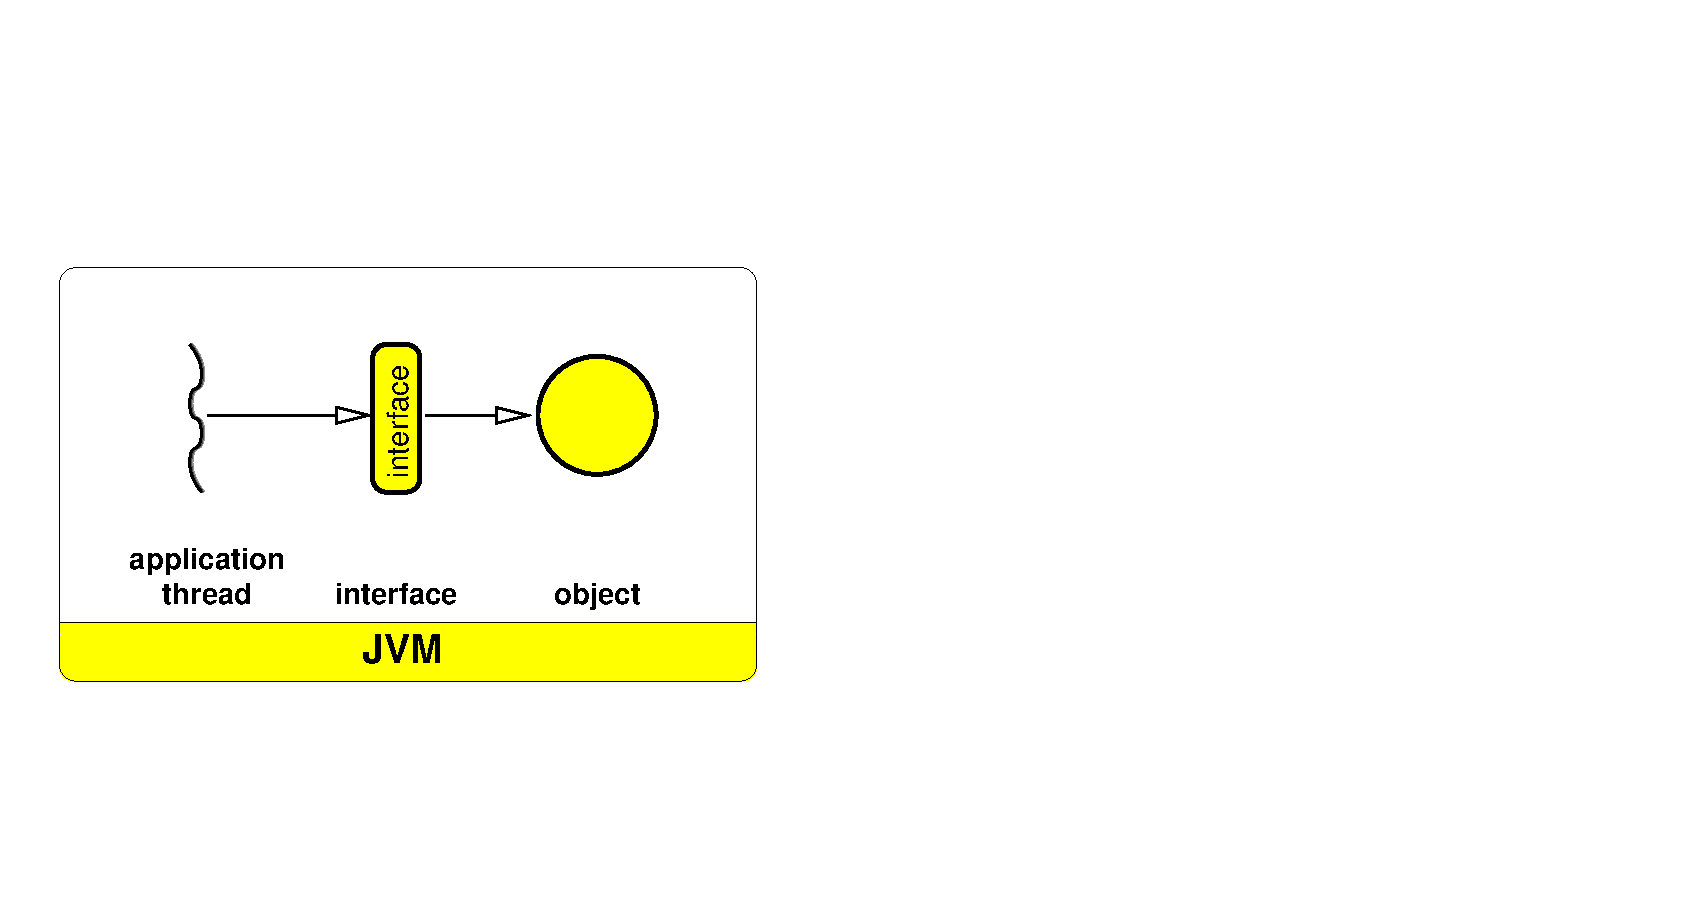
\includegraphics[width=0.7\textwidth]{normal.eps}
\end{center}
\caption{A normal invocation.}
\label{normal-fig}
\end{figure}

To turn the example of Figure~\ref{normal-fig} into a distributed RMI invocation,
some small modifications must be made to the program. The interface
must be turned into a remote interface by extending java.rmi.Remote,
and the object must be turned into a remote object by extending
java.rmi.UnicastRemoteObject. The rmic compiler, which is part of the
Java Developer Kit (JDK), can then generate the required communication
code. This code consist of two objects, a 'stub' and a 'skeleton', as
shown in Figure~\ref{rmi-fig}.

\begin{figure}[t]
\begin{center}
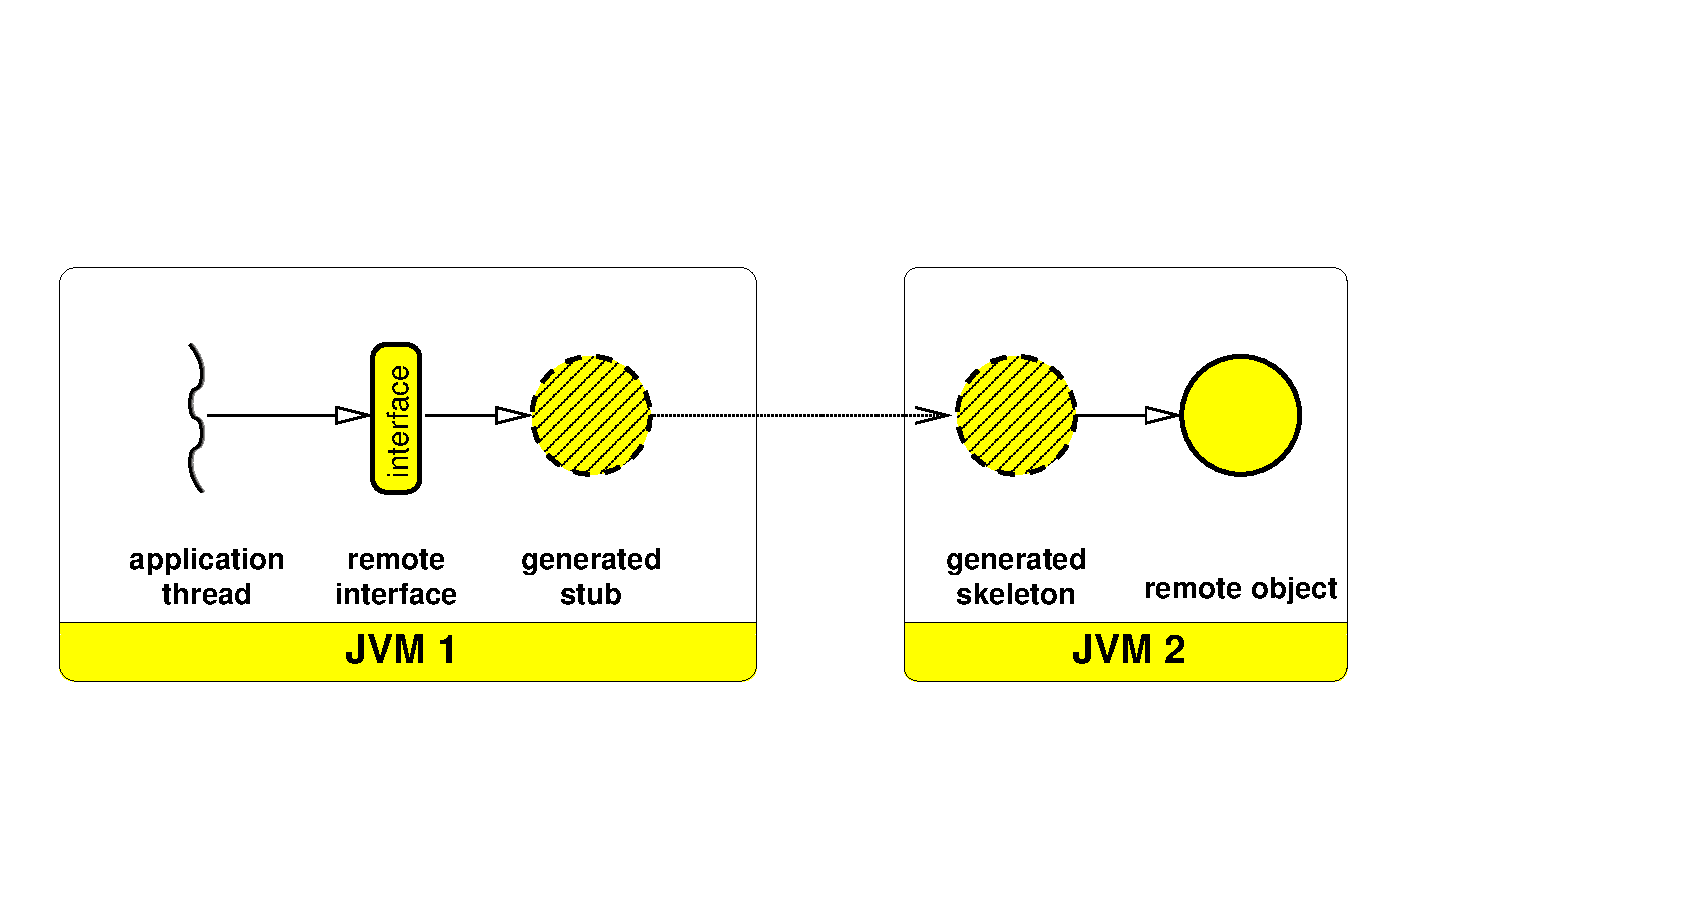
\includegraphics[width=0.7\textwidth]{rmi-abstract.eps}
\end{center}
\caption{A remote invocation with RMI.}
\label{rmi-fig}
\end{figure}

The stub object implements the application interface, and contains
code to forward any method invocations it receives to a skeleton
object on another JVM. The skeleton object contains code to receive
these invocations, and perform them on the object. It then sends the
results back to the stub, which returns them to the waiting
application thread.  Although RMI is not completely transparent, only
small modifications to the application are required. Furthermore, the
programmer does not have to write any communication code (this is
generated by rmic), making RMI easy to use. Unfortunately, the way in
which method invocations are handled in RMI is fixed. After the stub
forwards the invocation to the skeleton, it waits for a reply message
before continuing. The skeleton must therefore always send a reply
back to the stub (even if the method has no result. Furthermore, a
stub in RMI always serves as a 'remote reference' to a single object,
which can not be changed once the stub has been created.

There is very little difference between the usage of Sun RMI and Ibis
RMI. The programs are exactly the same, you only have to compile them
with Ibis \texttt{rmic} instead of the Sun \texttt{rmic}. 

%\remark{TODO limitations/restrictions.}


\mysubsection{Compiling and running an Ibis RMI program}

Before running an Ibis RMI application it must be compiled.
Using \emph{ant}, this is quite easy. Here is an example build.xml file:

\begin{quote}
\begin{verbatim}
<project
    name="Project name"
    default="build"
    basedir=".">

    <description>
    Ibis RMI application build.
    </description>

    <property environment="env" />
    <property name="ibis"   value="${env.IBIS_HOME}" />

    <property name="build"  location="build"/>

    <import file="${ibis}/build-files/apps/build-rmi-app.xml"/>
</project>
\end{verbatim}
\end{quote}

Again, we assume that the environment variable \texttt{IBIS\_HOME} reflects
the location of your Ibis installation.

Invoking \emph{ant build-sun} compiles a standard Java RMI version of
the application, leaving the class files in a directory called \texttt{build}.
Invoking \emph{ant build} compiles the application for Ibis RMI.
Running an Ibis RMI program is very much like running an Ibis application.

To test this for yourself, it is best to start with
an example, say \texttt{\$IBIS\_HOME/apps/rmi/tsp}. 
If you want to test your own application, it is easiest to just copy
the \texttt{build.xml} file from \texttt{\$IBIS\_HOME/apps/rmi/tsp}, and adapt it for your
application. 
To compile the TSP example, please type
\begin{verbatim}
$ ../../../ant clean build-sun
\end{verbatim}
\noindent
Now, this example application will be compiled with Sun RMI.
Running the TSP example with Sun RMI can be done as follows. Run the command
\begin{verbatim}
$ java \
    -cp $IBIS_HOME/build/ibis.jar:$IBIS_HOME/3rdparty/log4j-1.2.9.jar:build \
    -Dibis.pool.total_hosts=2 -Dibis.pool.server.host=localhost \
    Server table_15.1
\end{verbatim}
\noindent
in two seperate shells. The application should now run ``in parallel''
on the local machine. Alternatively, you can use the \emph{ibis-run} script:

\begin{verbatim}
$ $IBIS_HOME/bin/ibis-run -nhosts 2 -hostno 0 Server table_15.1
\end{verbatim}

\noindent
in the first shell, and

\begin{verbatim}
$ $IBIS_HOME/bin/ibis-run -nhosts 2 -hostno 1 Server table_15.1
\end{verbatim}

\noindent in the second.

The TSP application uses the \texttt{PoolInfo}
class that comes with Ibis. This utility class can be used both with
Sun RMI and Ibis RMI. This class is there for convenience, it provides
some methods to retrieve the number of processors in the parallel run
and the ranks of the participating processors. Because this class
comes with Ibis, \texttt{ibis.jar} has to be in the classpath, even
when running with Sun RMI.  The \texttt{PoolInfo} class needs the
\texttt{ibis.pool.total\_hosts} and \texttt{ibis.pool.server.host}
properties in order to be able to assign ranks to processors. The
pool server is started automatically when you start an ibis nameserver
with the \texttt{ibis-namesever} script (in the case of this example, this is done automatically).

Now, we can run the same application with Ibis RMI as follows.
Remember that you first have to recompile it with the Ibis rmic:
\begin{verbatim}
$ ../../../ant clean build
\end{verbatim}
\noindent
Now we can run it by typing the following command in two seperate shells:
\begin{verbatim}
$ java \
    -cp $IBIS_HOME/build/ibis.jar:$IBIS_HOME/3rdparty/log4j-1.2.9.jar:build \
    -Dibis.pool.total_hosts=2 -Dibis.pool.server.host=localhost \
    -Dibis.name_server.host=localhost -Dibis.name_server.key=bla \
    Server table_15.1 
\end{verbatim}
\noindent

This should produce the same result as the Sun RMI test.
If you want to run the application with the \texttt{ibis-run} script,
you can use the same commandline as with the Sun RMI test.

\mysection{The GMI (Group Method Invocation) System}
\label{gmi-sec}

For many parallel and distributed applications, the simple synchronous
unicast communication model (one-to-one communication with a reply)
offered by RMI is inadequate.  Applications often require more
different, more complex forms of communication, such as asynchronous
unicast (one-to-one communication without a reply), broadcast
(one-to-all communication), multicast (one-to-many communication), or
data reduction operations (where data must be collected from multiple
machines).  Although these alternative forms of communication can be
implemented using RMI, this is often complex and inefficient. For
example, a simple way to implement multicast is to perform multiple
RMI calls, one after the other. Unfortunately, this is very
inefficient, since each RMI must wait until the previous RMI has
finished completely, including waiting for the (unused) result to be
returned. More efficient implementations use threads to perform
multiple RMIs simultaneously or create distributed multicast trees
which use multiple machines to forward calls. These implementations
are complex, however, and often suffer from performance problems
caused by the synchronous nature of RMI.  In Ibis, we offer a new
programming model called GMI (Group Method Invocation). GMI is an
extension of RMI designed to be flexible enough to express the complex
forms of communication needed by many parallel
applications. Nevertheless, GMI is as easy to use as RMI, hiding the
complex details of the communication in its implementation. The
flexible model of GMI also allows its implementation to use efficient
communication algorithms for multicast, data reduction, etc. The GMI
model will be explained in detail below.


\mysubsection{The GMI model}

The GMI model generalizes the RMI model in three ways. First, it
introduces the notion of a 'group', a set of objects which all
implement the same interface. The objects in a group may be
distributed over a number of JVMs. A group can be addressed using a
single 'group reference'. An example is shown in Figure~\ref{gmi-fig}, where an
application thread uses a single group reference to address a group of
two objects (on different JVMs).

\begin{figure}[t]
\begin{center}
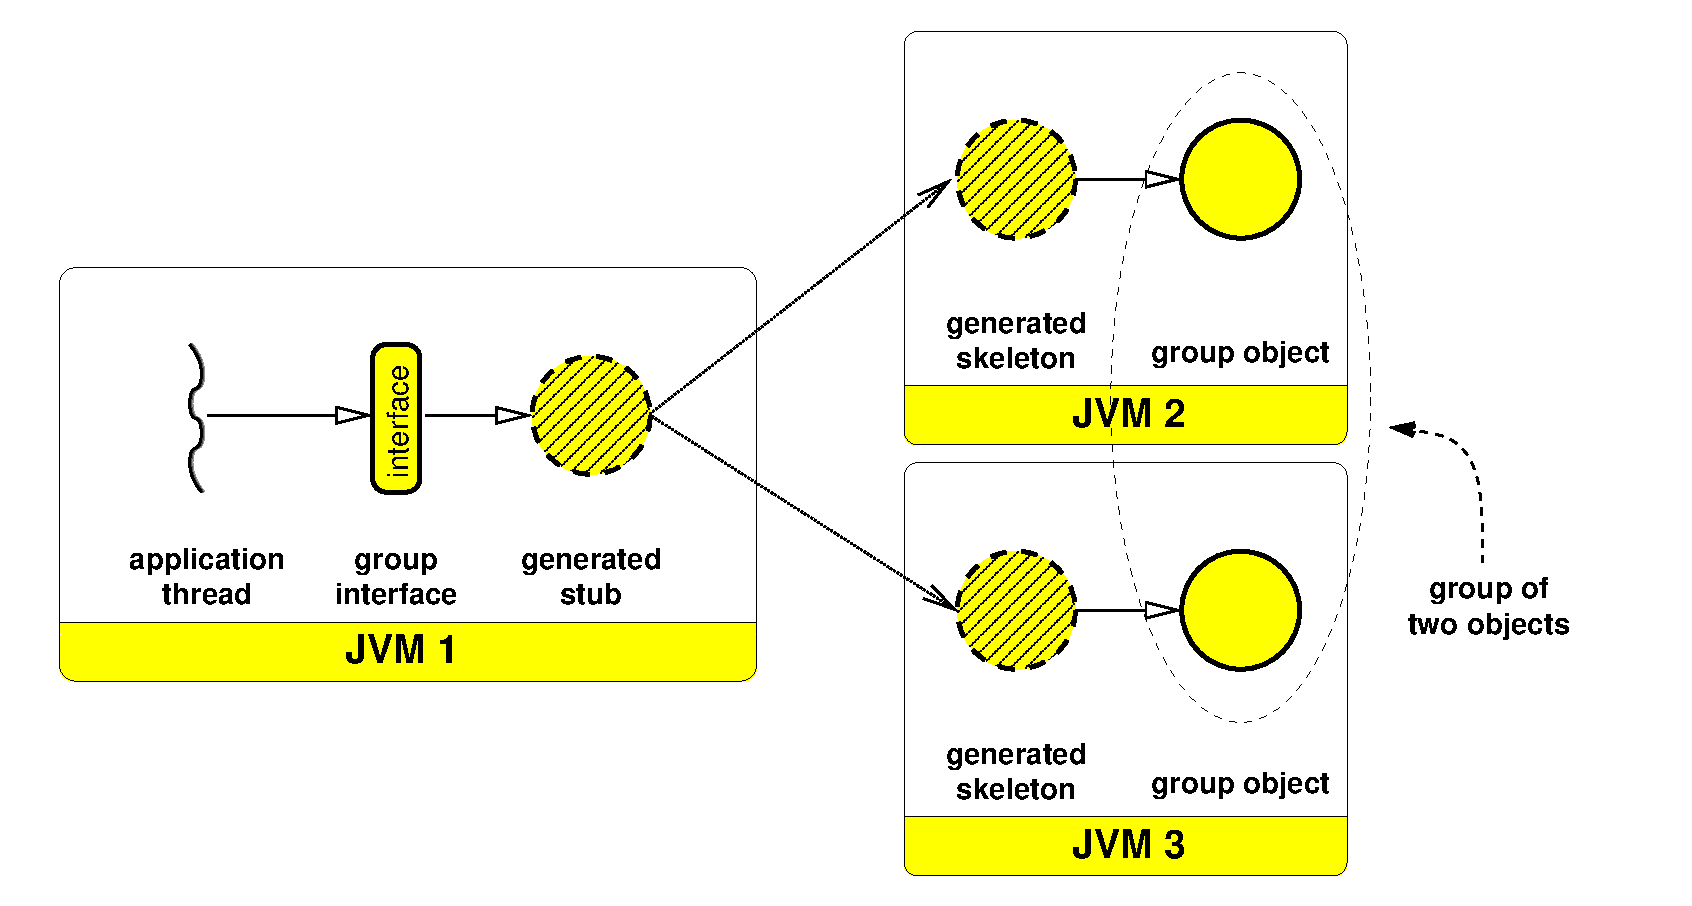
\includegraphics[width=0.7\textwidth]{gmi-abstract.eps}
\end{center}
\caption{A group invocation with GMI.}
\label{gmi-fig}
\end{figure}

Like RMI, GMI uses compiler generated stub and skeleton objects which
implement the necessary communication code. The application programmer
does not have to write any communication code. Unlike RMI, however,
GMI does not only generate code for synchronous unicast
communication. Instead, many different types of communication code are
generated, both for sending of method invocations and for returning of
results. This is the second generalization introduced by GMI.
Finally, through a simple API, the programmer can configure at run
time which type of communication should be used to handle each
individual method of a group reference. This API will be explained in
more detail in the next section. Different ways of forwarding the
invocation and handling the results can be combined, giving a rich
variety of communication mechanisms. By configuring the methods at run
time, the communication behavior of the application can easily be
adapted to changing requirements.

The following types of method invocation forwarding are currently
supported by GMI:
\begin{itemize}
\item{single invocation:}
The method invocation is
forwarded to a single object of the group, identified via a rank.
\item{group invocation:}
The invocation is forwarded to every object in the
group.
\item{personalized group invocation:}
The invocation is forwarded to
every object in the group, while the parameters are personalized for
each destination using a user-defined method.
\item{combined invocation:}
Multiple application threads (possibly on multiple JVMs) invoke the
same method on the same group. These invocations are combined into a
single invocation using a user-defined method. This single invocation
is forwarded to the group using one of the three other forwarding
schemes.
\end{itemize}

The following types of method result handling are currently supported
by GMI:
\begin{itemize}
\item{discard results:}
No results are returned at all (including
exceptions).
\item{return one result:}
A single result is returned,
preselected via a rank if neccesary.
\item{forward results:}
All results are
returned, but they are forwarded to a user-defined object rather than
being returned to the invoking thread.
\item{combine results:}
Combine all
results into a single one using a user-defined method. The combined
result is returned to the invoker.
\item{personalize result:}
A result
produced by one of the other result handling schemes is personalized
using a user-defined method before being returned to each of the
invokers (this is useful when a combined invocation is used).  The
four different forwarding schemes and five different result handling
schemes can be combined orthogonally, resulting in a wide variety of
useful communication patterns.  
\end{itemize}

\mysubsection{Hello world in GMI}

We will now show a
step by step example of how a GMI application can be written. The
first step is to create an interface which will define the methods
which can be invoked on the group of objects. Like in RMI, we use a
special 'marker interface' to 'mark' group interfaces. Any interface
extending ibis.gmi.GroupInterface will be recognized by the Ibis
compiler as being a group interface. The Ibis compiler will then
generate a stub object which contains the necessary communication
code.

\begin{quote}
\begin{verbatim}
interface Example extends ibis.gmi.GroupInterface {
   public void put(String message);
   public String get();
}
\end{verbatim}
\end{quote}
\noindent

In the example above, the 'Example' interface is turned into a group
interface by extending ibis.gmi.GroupInterface. It defines just two
methods, put, which can be used to store a string, and get which can
be used to retrieve a stored string.  After creating the group
interface, an implementation of this interface is be created. This
implementation object must implement the Example interface, and extend
the ibis.gmi.GroupMember object, which contains some basic
functionality needed to be part of a group (this is similar to the
UnicastRemoteObject used in RMI).

\begin{figure}[t!]
\small{
\begin{quote}
\begin{verbatim}
import ibis.gmi.GroupMember;

class Implementation extends GroupMember implements Example {

   private String message = null;

   public synchronized void put(String message) {
      this.message = message;
      notify();
   }
   
   public synchronized String get() { 
      while (message == null) { 
         wait();
      }       
      return message;
   } 
}
\end{verbatim}
\end{quote}
}
\caption{Implementing a group object with GMI.}
\label{gmi-1}
\end{figure}

In this implementation, shown in Figure~\ref{gmi-1}, the put method stores the
string it receives in the object, from where it can be retrieved using
the get method. The standard synchronization primitives synchronized,
wait, and notify are used to prevent the get from returning before the
string is available.  Next, we will create an simple example
application, BroadcastExample, which will use the group object. The
source code is shown in Figure~\ref{gmi-2}. This application is parallel; it is
designed to be started simultaneously on multiple JVMs.

\begin{figure}[t!]
\small{
\begin{quote}
\begin{verbatim}
import ibis.gmi.*;

class BroadcastExample {

   public static void main(String[] args) {
      int size = Group.size();
      int rank = Group.rank();

      if (rank == 0) {
         // JVM 0 creates a new group. 
         Group.create("ExampleGroup", Example.class, size);
      } 

      // All JVMs create an implementation object.
      Implementation impl = new Implementation();
   
      // And join the group
      Group.join("ExampleGroup", impl);

      if (rank == size-1) { 
         // The last JVM retrieves a group reference
         Example group = (Example) Group.lookup("ExampleGroup");

         // Then configures 'put' to be forwarded to the whole group
         GroupMethod m = Group.findMethod(group, "void put(java.lang.String)");
         m.configure(new GroupInvocation(), new DiscardReply());

         // Now invoke a method on the group
         group.put("Hello world!");
      } 

      // All JVMs can now retrieve the data using a local(!) call
      String message = impl.get();        
      System.out.println(message);

      // Done   
      Group.exit();
   }
} 
\end{verbatim}
\end{quote}
}
\caption{An example GMI application that uses a group object.}
\label{gmi-2}
\end{figure}

The main method of the application starts by invoking Group.size and
Group.rank, two utility methods of GMI which can be used to find out
how many JVMs are available (size), and what number is assigned to the
current JVM (rank).  The JVM with rank 0 then creates a new group
using Group.create. This group will have the name ExampleGroup, use a
group interface of the type Example and will contain 'size'
objects. Each JVM then creates it's own Implementation object, and
adds it to the group using the Group.join method. Group.join will
block until all 'size' objects have been added to the group.  The last
JVM (with rank 'size-1') then retrieves a group reference using
Group.lookup. This method will return a stub generated by the Ibis
compiler. This stub contains the communication code necessary to
communicate with the objects in the group. Because the stub implements
the Example interface, normal invocations of the put and get methods
can be used and no communication code needs to be written by the
programmer. But before the methods can be invoked, the group stub must
first be configured.  All methods in a group stub can be configured
separately. In this example we will only use the put method. To
configure put, we first perform a lookup of the method using
Group.findMethod. A GroupMethod object will be returned, which
represents the put method of the stub.  Using the configure method in
this GroupMethod object, it can be specified how the invocations of
the put method should be handled. For this purpose the configure
method takes two parameters, one describing how the invocation must be
forwarded to the group, and one describing how the replies should be
returned. In the example application we use GroupInvocation and
DiscardReply, which indicates that invocations of put will be
forwarded to all objects in the group, and that no replies will be
returned.  After the configuration is completed, the last JVM invokes
the put method. The method invocation is then forwarded to all object
in the group. All JVMs then retrieve their local copy of the string by
directly invoking the get method on their implementation objects.


\mysubsection{Compiling and running a GMI program}

Before running a GMI application it must be compiled.
Using \emph{ant}, this is quite easy. Here is an example build.xml file:

\begin{quote}
\begin{verbatim}
<project
    name="Project name"
    default="build"
    basedir=".">

    <description>
    GMI application build.
    </description>

    <property environment="env" />
    <property name="ibis"   value="${env.IBIS_HOME}" />

    <property name="build"  location="build"/>

    <import file="${ibis}/build-files/apps/build-gmi-app.xml"/>
</project>
\end{verbatim}
\end{quote}

Again, we assume that the environment variable \texttt{IBIS\_HOME} reflects
the location of your Ibis installation.

Invoking \emph{ant build} compiles the application for GMI.

Running a GMI program is very much like running an Ibis application.
See Section \ref{Compiling and Running an Ibis Application} for details.


\mysection{Further Reading}

The Ibis web page
{\html {\htmladdnormallink{http://www.cs.vu.nl/ibis/publications.html} {http://www.cs.vu.nl/ibis/publications.html}}}
{\latex {http://www.cs.vu.nl/ibis/publications.html}}
contains links to various Ibis papers.
The best starting point might be \\
{\html {\htmladdnormallink{http://www.cs.vu.nl/~rob/papers/cpe03.ps.gz} {http://www.cs.vu.nl/\~{}rob/papers/cpe03.ps.gz}}}
{\latex {http://www.cs.vu.nl/\~{}rob/papers/cpe03.ps.gz}}, which gives a high-level description of the stucture of the Ibis system.
It also gives some low-level and high-level benchmarks of the different Ibis implementations.

The \emph{docs/api} subdirectory of the Ibis installation provides
documentation for each class and method in the Ibis API (point your favorite
HTML viewer to docs/api/index.html in the Ibis installation).
The Ibis API is also available
\html{\htmladdnormallink{on-line}{http://www.cs.vu.nl/ibis/api/index.html}.}
\latex{on-line at http://www.cs.vu.nl/ibis/api/index.html.}

\end{document}
